\subsection{Transfer to dense prediction}
Transfer learning for dense prediction is critical especially since obtaining pixel-level labels can be costly. In this section, we investigate the quality of captured geometric and spatial information by the \chonk model (trained using image-level classification objective) on semantic segmentation and monocular depth estimation tasks.


\subsubsection{Semantic segmentation}
\paragraph{Experimental setup.}
We evaluate \chonk as a backbone in semantic segmentation on three benchmarks: ADE20K~\citep{zhou2017scene}, Pascal Context~\citep{mottaghi2014role} and Pascal VOC~\citep{everingham2010pascal}.
%Recent works have shown that plain ViT architectures can be used for dense recognition tasks~\citep{strudel2021segmenter,minderer2022simple}.
We analyze the performance in two scenarios:
first, using a limited amount of data for transfer;
second (in~\cref{app:semantic_segmentation}), comparing end-to-end fine-tuning \textit{versus} a frozen backbone with either a linear decoder~\citep{strudel2021segmenter} or UperNet~\citep{xiao2018unified}.
The number of additional parameters ($\approx1$M for linear and $\approx783$M for UperNet) is negligible compared to the size of the backbone. We use a fixed resolution ($504$px) and report single scale evaluation.

\paragraph{Results.}
We compare \chonk to the ViT-L of DeiT-III~\citep{touvron2022deit} and ViT-G of \citet{zhai2022scaling}, when only a fraction of the ADE20k semantic segmentation data is available. % during transfer.
We use the linear decoder and end-to-end fine-tuning.
From \cref{tab:semseg_fewshot}, we observe that our \chonk backbone transfers better when seeing only few segmentation masks.
For example, when fine-tuning with only 1200 images (i.e.\ $1/16$) of ADE20k training data, we reach a performance of 44.7 mIoU, an improvement of $+8.6$ mIoU over DeiT-III Large~\citep{touvron2022deit} and $+2.3$ mIoU over ViT-G~\citep{zhai2022scaling}.
When transferring with more data, the performance of ViT-G and \chonk converge.

\begin{table}[t]
    \caption{
      %\textbf
      Fewshot semantic segmentation on ADE20k, when only a fraction of the training set is used.
We report mean IoU for semantic segmentation on the validation set.
%for \chonk, ViT-L~\citep{touvron2022deit} and ViT-G~\citep{zhai2022scaling}. % the citations are already in the table
% Only a fraction
% either $1/16$, $1/8$, $1/4$, $1/2$ or $1$ (full)
% of the ADE20k training images are used. % for fine-tuning.
Transfer is done with end-to-end fine-tuning and a linear decoder, following~\citet{strudel2021segmenter}.
We average over 3 runs.
}
\centering
\small
  \setlength{\tabcolsep}{4pt}
      \resizebox{.6\textwidth}{!}{%
    \begin{tabular}{@{} l c c c c c @{}}
      \toprule
	    Fraction of ADE20k train data      & $1/16$ & $1/8$ & $1/4$ & $1/2$ & $1$ \\
      \midrule
      ViT-L~\citep{touvron2022deit} & 36.1 & 41.3 & 45.6 & 48.4 & 51.9 \\
      ViT-G~\citep{zhai2022scaling} & 42.4 & 47.0 & 50.2 & 52.4 & \textbf{55.6} \\
      \chonk (Ours) & \textbf{44.7} & \textbf{47.2} & \textbf{50.6} & \textbf{52.5} & 54.9 \\
      \bottomrule
 \end{tabular}
 }
    \label{tab:semseg_fewshot}
\end{table}



\subsubsection{Monocular depth estimation}
% In order to investigate the geometric information retained by \chonk's features, we evaluate the frozen pre-trained model on a monocular depth estimation task.
% To investigate how much geometry information is retained in the features learned by \chonk we evaluate the frozen backbone on a monocular depth estimation task.

\paragraph{Experimental setup.}
%\todo{shorten to 1 paragraph}
We largely mirror the set-up explored in \citet{ranftl2021vision} and train their Dense Prediction Transformer (DPT) on top of frozen \chonk backbone features obtained from the Waymo Open real-world driving dataset~\citep{sun2020scalability}.
Here we use only a single feature map (of the last layer) to better manage the high-dimensional ViT features.
We also explore a much simpler ``linear'' decoder as a lightweight readout.
In both cases we predict $\log(1 + \text{depth})$ obtained from sparse LiDAR as the target and use Mean Squared Error (MSE) as the decoder training loss. 
We quantify performance using standard depth estimation metrics from the literature~\citep{hermann2020self, eigen2014depth} and also report MSE. We use a resolution of $224\times224$. 
Remaining details are deferred to \Cref{app:de}.

% We use the Waymo Open real-world driving dataset~\citep{sun2020scalability}, which is composed of $1280\times1920$ resolution video frames obtained from a multi-camera system, recording videos of length $20$ seconds at $10$ frames per second (fps).
% We train a decoder on top of frozen \chonk backbone features on training set frames and evaluate it on the first 5120 validation set frames from the front facing camera, sub-sampled at 5 fps and at $224\times224$ resolution.
% We compute sparse depth maps as targets by projecting the corresponding ground truth LiDAR points to the camera frame.

% For the decoder, we largely mirror the set-up explored in \citet{ranftl2021vision} and use their Dense Prediction Transformer (DPT) with minor differences (see \Cref{app:de}).
% To better manage the high-dimensional ViT features, we use the same feature map (of the last layer) in each of the four reassemble blocks.
% We also explore a much simpler ``linear'' decoder as a lightweight readout complementary to our DPT experiments.  
% Details of its architecture are deferred to \Cref{app:de}.
% In both cases we predict $\log(1 + \text{depth})$ as the target and use Mean Squared Error (MSE) as the decoder training loss. 

% We quantify performance using the following standard depth estimation metrics from the literature~\citep{hermann2020self, eigen2014depth}, and also report the MSE loss on the validation set:
% AbsRel measures the mean absolute error between the ground truth and predicted depth relative to the ground truth, while the inlier fraction metrics ($\delta$) measure the fraction of valid pixels within a certain 
% percentage
% from ground truth.
% All metrics were measured after undoing the log transformation.


\begin{figure}[tbp]
    \centering
    \subfigure[Semantic segmentation]{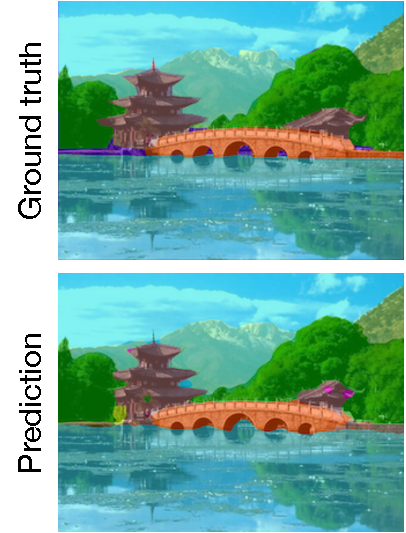
\includegraphics[width=0.315\linewidth]{figs/semseg/semantic_seg.pdf}}\quad\quad \quad\quad
    \subfigure[Depth estimation]{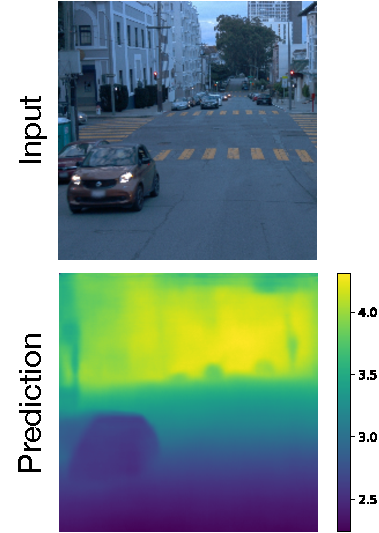
\includegraphics[width=0.2955\linewidth]{figs/depth_prediction/depth_estimation.pdf}}
    \caption{Dense prediction from frozen \chonk features.}
    \label{fig:dense_prediction}
% \vspace{-10pt}
\end{figure}

\begin{table}[t]
\caption{%\textbf
{Monocular depth estimation} from frozen ViT features using different decoders on the Waymo Open dataset.}
\centering
\small
\setlength{\tabcolsep}{4pt}
\resizebox{.55\textwidth}{!}{%
\begin{tabular}{@{} ll ccccc  @{}}
  \toprule
   & & & & \multicolumn{3}{c}{$\delta$ $\uparrow$} \\
   \cmidrule(l{2pt}r{2pt}){5-7}
    & Model      & MSE $\downarrow$ & AbsRel $\downarrow$ & $< 1.1$& $< 1.25$& $< 1.25^2$\\
  \midrule
  \multirow[c]{3}{*}{\rotatebox{90}{DPT}} & ViT-L & 0.027 & 0.121 & 0.594 & 0.871 & 0.972 \\ % xid/50851792
  & ViT-e & 0.024 & 0.112 & 0.631 & 0.888 & 0.975 \\ % xid/50851464
  & \chonk & \textbf{0.021} & \textbf{0.095} & \textbf{0.702} & \textbf{0.909} & \textbf{0.979} \\ % xid/48459029
  \midrule
  \multirow[c]{3}{*}{\rotatebox{90}{Linear}} & ViT-L & 0.060 & 0.222 & 0.304 & 0.652 & 0.926 \\ % xid/50902199
  & ViT-e & 0.053 & 0.204 & 0.332 & 0.687 & 0.938 \\ % xid/50901568
  & \chonk & \textbf{0.039} & \textbf{0.166} & \textbf{0.412} & \textbf{0.779} & \textbf{0.960} \\ % xid/50861091
  \bottomrule
\end{tabular}
}
\label{tab:depth_estimation}
% \vspace{-10pt}
\end{table}



\paragraph{Results.}
\Cref{tab:depth_estimation} summarizes our main findings.
From the top rows (DPT decoder), we observe that using \chonk features yields the best performance (across all metrics) compared to different backbones. By comparing the \chonk backbone to ViT-e (a smaller model but trained on the same data as \chonk) we find that scaling the architecture improves performance. Further, comparing the ViT-e backbone to ViT-L (a similar architecture to ViT-e but trained on less data) we find that these improvements also come from scaling the pre-training data. These findings demonstrate that both the greater model size and the greater dataset size contribute substantially to the improved performance.
%, and we find that both the greater model size and the greater dataset size contribute substantially to the improved performance from comparing ViT-L (smaller model trained on smaller data) and ViT-e (smaller model trained on the same data).
%In absolute terms, the scores obtained using \chonk appear competitive with results reported in the literature on other driving datasets.
%, indicating that we obtained good performance on Waymo Open.\todo{@gamal are there no numbers on Waymo anywhere that we can compare to roughly?}
Using the linear decoder, it can be observed again that using \chonk features yields the best performance.
% The greatly improved scores when using a DPT decoder suggest that while enough geometric information is retained in the ViT features, only some of it is available at the surface level.  
The gap between DPT and linear decoding suggests that while enough geometric information is retained in the ViT features, only some of it is available for a trivial readout.
We report qualitative results in \Cref{fig:dense_prediction} and \Cref{fig:dpt_depth_predictions_full,fig:dpt_depth_predictions_full_error} in \cref{app:de}.

% Xolab for the numbers: https://colab.corp.google.com/drive/1IjaxfaLJBNvmgLJXkicHggwyNL7uxpZ-?usp=sharing 


